 \centering
        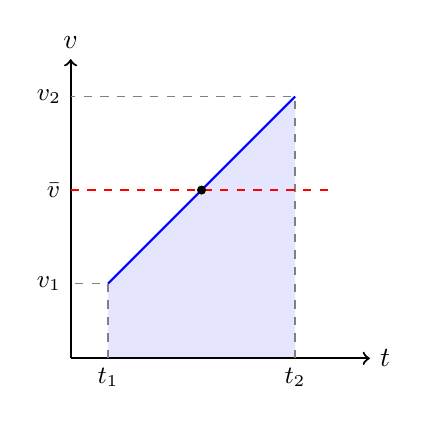
\begin{tikzpicture}[scale=0.95]
            % Área sombreada (Trapézio)
            \fill[blue, opacity=0.1] (0.5,0) -- (0.5,1) -- (3,3.5) -- (3,0) -- cycle;

            % Eixos
            \draw[->,thick] (0,0) -- (4,0) node[right] {$t$};
            \draw[->,thick] (0,0) -- (0,4) node[above] {$v$};
            
            % Reta do MRUV
            \draw[blue, thick] (0.5,1) -- (3,3.5);
            
            % Linhas de projeção
            \draw[dashed, gray] (0.5,0) node[below, black] {\small $t_1$} -- (0.5,1) -- (0,1) node[left, black] {\small $v_1$};
            \draw[dashed, gray] (3,0) node[below, black] {\small $t_2$} -- (3,3.5) -- (0,3.5) node[left, black] {\small $v_2$};
            
            % Linha da Velocidade Média
            \draw[red, thick, dashed] (0,2.25) node[left, black] {\small $\bar{v}$} -- (3.5,2.25);
            
            % Marcação do ponto médio
            \filldraw[black] (1.75,2.25) circle (1.5pt);
        \end{tikzpicture}
        
        \vspace{0.5em}
        % Usamos raggedright ou centering para evitar o esticamento das palavras (Underfull \hbox)
        \begin{minipage}{0.65\textwidth}
            \captionsetup{type=figure, name=Gráfico, hypcap=false}
            \captionof{figure}{Interpretação geométrica da velocidade média.}
            \label{graf:v_media_tikz}
        \end{minipage}